\documentclass{article}
\usepackage[pdftex]{graphicx}
\usepackage{hyperref}

\usepackage[utf8]{inputenc}
\usepackage[T1]{fontenc}
\usepackage[frenchb]{babel}
\usepackage{float}

\begin{document}

\title{Projet Recherche d'Information web \\- \\
Moteur de Recherche Ad-hoc de documents}
\author{Romain Catajar}

\maketitle

\begin{abstract}
Ce rapport présente les performances et choix d’implémentation de mon moteur de recherche sur la collection CACM. Plus particulièrement, j'analyse les résultats de mes modèles booléen et vectoriel par rapport aux recherches de référence fourni avec la collection et propose quelques pistes d’améliorations que je n'ai pas eu le temps d’implémenter.
\begin{center}
\url{https://github.com/rcatajar/recherche-web-ecp}
\end{center}
\end{abstract}


\section{Installation et utilisation du moteur de recherche}
En plus d’être normalement joint à ce rapport, le code de mon moteur de recherche est disponible sur GitHub, a l'adresse \url{https://github.com/rcatajar/recherche-web-ecp}


Le code nécessite Python 2.7, la librairie \texttt{NLTK} (\url{http://www.nltk.org/}) ainsi que les packages \texttt{stopwords}, \texttt{punkt} et \texttt{snowball\_data} de \texttt{NLTK}. Pour installer le moteur, il suffit de cloner ou de télécharger le contenue du dépôt. Des instructions plus précises sont disponibles sur GitHub si besoin.


L'utilisation de moteur de recherche se fait en exécutant les fichiers python dans un terminal. Deux commandes sont disponibles (le reste des fichiers correspondant au fonctionnement interne du moteur, présenté dans la partie suivante):
\begin{itemize}
    \item \texttt{python search.py} lance l'interface de recherche dans laquelle il est possible de choisir un modèle et d'effecteur des recherches dans la collection.
    \item \texttt{python evaluation.py} exécute toutes les recherches de référence fourni avec la collection, analyse les résultats et affiche différentes métriques de performance dans le terminal.
\end{itemize}


\section{Implémentation et fonctionnement du moteur}
Le code a été écrit en python dans le but d’être relativement facile à comprendre et est commenté exhaustivement en Français. Cette partie présente le fonctionnement général du moteur (du parsing de la collection a l’exécution d'une recherche), sans trop rentrer dans les détails de l’implémentation de chaque classe ou méthode (les méthodes et fichiers correspondants a chaque étapes seront indiqués pour permettre d'aller facilement regarder les détails dans le code directement).

\subsection{Parsing de la collection CACM}
Le parsing de la collection est effectué dans la classe \texttt{CACMCollection} du fichier \texttt{collection.py}. A instanciation, la classe ouvre le fichier contenant la collection, sépare les documents et pour chaque document, crée un objet \texttt{CACMDocument} (fichier \texttt{documents.py}) et charge chaque ligne du document dans le bon attribut (auteur, titre, résume et mots clés) en fonction des marqueurs.

\subsection{Indexation}
L'indexation est effectué par la classe \texttt{Index} du fichier \texttt{index.py}. L'index est instancié avec une série de documents, et il est possible d'en rajouter plus tard. On ajoute ensuite chaque document a l'index (méthode \texttt{add\_document}) on commence par processer tout son texte (auteur + titre + résume + keywords) dans la méthode \texttt{\_text\_to\_words} pour obtenir une liste de tokens. Le processing effectue les étapes suivantes:
\begin{itemize}
    \item mise en minuscule
    \item tokenization: plutôt que de juste séparer a chaque espace, j'ai utilisé la méthode \texttt{word\_tokenize} de \texttt{nltk} qui permet de séparer les mots de manière un peu plus précise (en utilisant l'algorithme \texttt{punkt sentence tokenizer} et en indiquant la langue du texte)
    \item retrait des mots courants: en plus de retirer les mots courants données dans la collection, je retire également les mots les plus courants de la langue anglaise (fourni par \texttt{nltk})
    \item stemming: finalement on ne garde que la racine des mots, pour deux mots ayant la même racine (par exemple verbe a l’infinitif et verbe conjugue, ou mot au singulier et au pluriel) ait le même token. J'ai pour cela utiliser le \texttt{SnowballStemmer} fourni par \texttt{nltk}
\end{itemize}


A partir de ces tokens on construit l'index (stocké dans \texttt{document\_index}), de la forme \texttt{\{id du document: \{token: nombre d’occurrence\}\}} et l'index inversé (stocké dans \texttt{word\_index}) de la forme \texttt{\{token: \{id du document: nombre d’occurrence\}\}}

On peux désormais à partir de ces indexes générer des vecteurs pour un document quand cela est nécessaire (pour la recherche vectorielle). Cela est fait dans la méthode \texttt{get\_document\_vector} qui supporte différent type de pondération en argument.


\subsection{Recherche booléenne}
La recherche vectorielle est implémenté dans le fichier \texttt{boolean\_search.py}, via la méthode \texttt{boolean\_search}. On part d'une query booléenne respectant les règles suivantes:

\begin{itemize}
    \item Opérateurs acceptés: (,  ),  AND,  OR,  NOT
    \item Un espace est considéré comme un AND
    \item Le nombre de parenthèses ouvertes doit matcher le nombre de parenthèses fermées
\end{itemize}

On commence par tokeniser cette query: on utilise le même processus que lors de l'indexation tout en faisant attention de ne pas toucher aux opérateurs. Une fois notre liste de token obtenue, on construit un arbre (methode \texttt{build\_query\_tree}) a partir de notre query (j'utilise pour cela une implémentation de l'algorithme \textit{Shunting-Yard} de \textit{Dijkstra} que j'ai trouvé sur internet). Notre arbre dispose de trois type de nœuds (le nom des nœuds correspond au nom de leur classe dans le code):

 \begin{itemize}
    \item \textbf{AndNode}: Nœud représentant un AND. le résultat de la recherche est l'intersection de ceux des nœuds fils
    \item \textbf{OrNode}: Nœud représentant un OR. le résultat de la recherche est l'union de ceux des nœuds fils
    \item \textbf{WordNode}: Nœud représentant un mot, sans enfant. le résultat de la recherche est l'ensemble des documents contenant ce mot dans notre index.
\end{itemize}

On peux ensuite obtenir facilement le résultat de la recherche en effectuant un parcours en profondeur de l'arbre.

Exemple d'arbre (pour la recherche \texttt{ NOT A OR (B AND C)}):

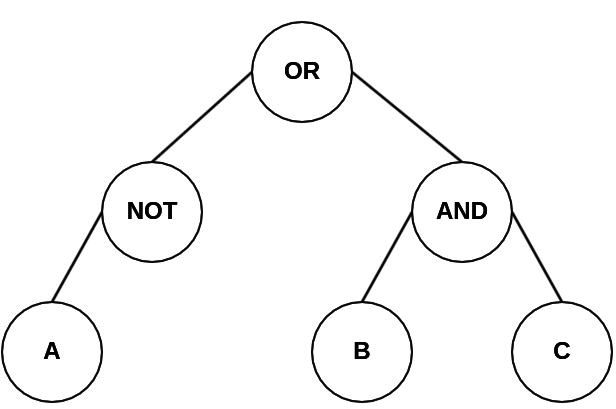
\includegraphics[scale=0.5]{grap.png}

\subsection{Recherche vectorielle}
La recherche vectorielle est implémenté dans le fichier \texttt{vectorial\_search.py}, via la méthode \texttt{vectorial\_search}. On part d'une query que l'on tokenize via notre index. A partir de la, l'index nous permet de calculer un vecteur de poids pour cette recherche.

On calcule ensuite le vecteur de poids de chaque document dans la collection et on calcule sa similarité avec celui de la recherche (via la mesure de similarité cosinus, implémenté dans la méthode \texttt{cosinus\_similarity}). On obtient ainsi une série de couple (document, similarité) que l'on ordonne par similarité.

Finalement, j'ai choisi de ne garder que les documents ayant une similarité avec la recherche d'au moins 15\% (mes tests ont montré que cela semble être une bonne valeur pour séparer les documents pertinents des documents très peu pertinents)

\subsection{Evaluation des performances}
Le fichier \texttt{evalution\_utils.py} contient différentes méthodes permettant d’évaluer la qualité et rapidité du moteur par rapport aux recherches de référence données avec la collection. J'ai implémenté des fonctions pour:
\begin{itemize}
\item importer les recherches et résultats de référence (méthodes \texttt{get\_queries} et \texttt{get\_expected\_results}) pour pouvoir leur comparer les résultats de ce moteur
\item calcul du temps d’exécution d'une instruction (méthode \texttt{time\_func}) pour pouvoir chronométrer les temps d'indexation et de recherche
\item différentes mesure de précision et de rappel: précision (avec ou sans ordre), average precision, rappel (avec ou sans ordre), R précision, mesure E, mesure F, calcul de moyenne (méthodes \texttt{precision}, \texttt{average\_precision}, \texttt{rappel}, \texttt{R\_precision}, \texttt{E\_measure}, \texttt{F\_measure} et \texttt{average})
\end{itemize}

\section{Performances et analyse des résultats}
Tous les résultats de cette partie ont été obtenue en exécutant le script \texttt{evaluation.py} sur mon ordinateur portable (processeur dual-core 2GHz et 8 Go de mémoire vive). Les résultats relatifs a la rapidité d’exécution peuvent évidement varier d'une machine à une autre, les mesures de performances devraient être identiques.

\subsection{Présentation des performances}
\subsubsection*{Indexation}
Le moteur parse la collection CACM en environ \textbf{0.2 seconde} et l'indexe en \textbf{6.5 secondes}. Une fois indexé, l'index en mémoire pèse environ \textbf{1 Méga octet}

\subsubsection*{Modèles de recherche}
Sont présentés ici les résultats moyens de moteur de recherches sur l'ensemble des recherches de référence fournies par la collection CACM

\begin{table}[H]
\centering
\label{my-label}
\begin{tabular}{r|c|c|}
\cline{2-3}
                                                                       & \textbf{Modèle Booléen}                                                           & \textbf{Modèle Vectoriel} \\ \hline
\multicolumn{1}{|r|}{\textbf{temps d’exécution moyen de la recherche}} & 0.02 s                                                                            & 0.02 s                    \\ \hline
\multicolumn{1}{|r|}{\textbf{précision (sans ordre) moyenne}}          & 0.26                                                                              & 0.32                      \\ \hline
\multicolumn{1}{|r|}{\textbf{rappel moyen}}                            & 0.08                                                                              & 0.22                      \\ \hline
\multicolumn{1}{|r|}{\textbf{R précision moyenne}}                     & \begin{tabular}[c]{@{}c@{}}non pertinent\\ (résultats non ordonnées)\end{tabular} & 0.54                      \\ \hline
\multicolumn{1}{|r|}{\textbf{F mesure moyenne}}                        & 0.04                                                                              & 0.20                      \\ \hline
\multicolumn{1}{|r|}{\textbf{E mesure moyenne}}                        & 0.96                                                                              & 0.80                      \\ \hline
\end{tabular}
\end{table}

\end{document}
